\subsection{Blockschaltbild}\label{subsec:Blockschaltbild}

Das Blockschaltbild soll die Funktionsweise der Cocktailmaschine veranschaulichen. Dabei wird unterschieden zwischen der Steuerelektronik (MCS) und den externen Komponenten wie Netzteil, Touchscreen (HMS), Beleuchtung (ML), Pumpen, Durchflussmessgeräte, Endschalter und Motor. Aufgrund dieses Blockschaltbildes werden in den folgenden Kapitel die Hauptkomponenten ausgewählt.

\begin{figure}[h!]
	\centering
	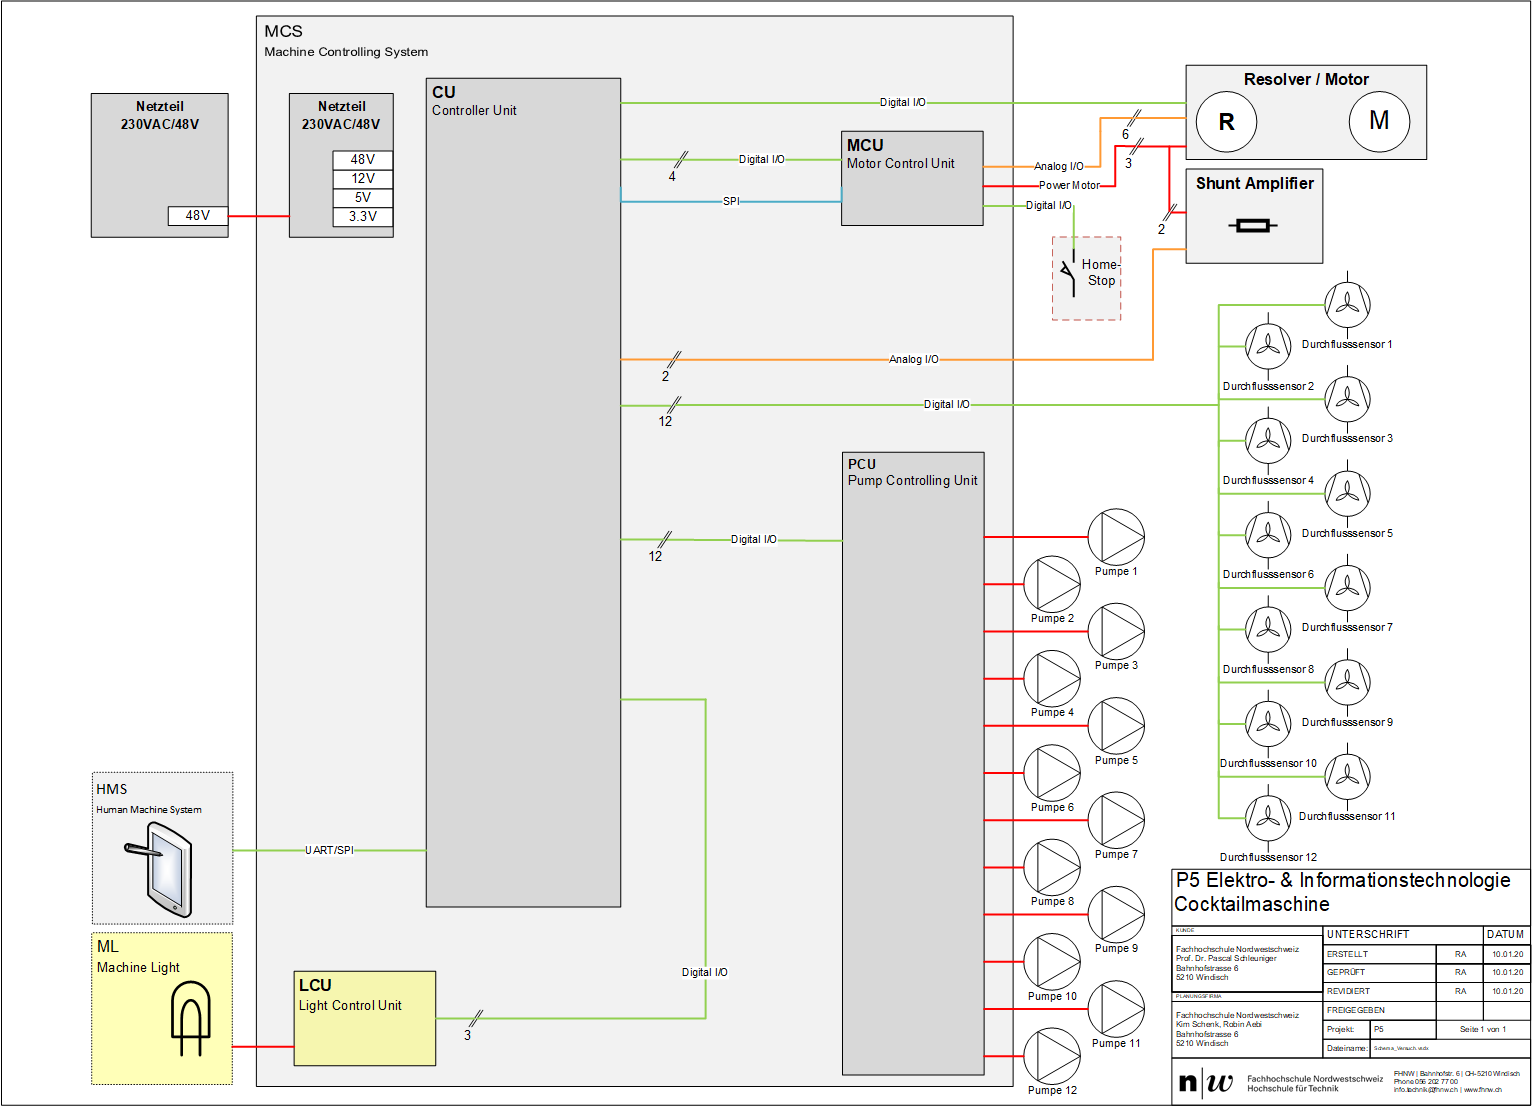
\includegraphics[angle=90, width=\textwidth]{graphics/P5-Blockschema.png}
	\caption{Blockschaltbild}
	\label{fig:Blockschaltbild}
\end{figure}  

\newpage  